\chapter{Implementation}

This chapter gives the implementation details for the design presented in Chapter \ref{design}. Code blocks are used at necessary places to give extensive details. The code written as part of the thesis can be accessed in the Github repository \cite{git_synccode}.

This implementation used the Genode OS framework 15.11 and was written in C++ to be compatible with the Genode operating system and the Fiasco.OC, which are both developed in C++. The following sections describe the module implementation.

The first aim was to find access to the ready queue of the scheduler from the Genode. The task was to find an L4 API, which has access to the ready queue and unfortunately there existed none. According to the l4-hackers, on Fiasco's API level, there is no interface to directly access the run queues of processors. The current APIs allow to set only the scheduling and CPU affinity parameters \cite{l4hack}. This forced the creation of a new API that gives access to read/write the kernel ready queue to the Genode or to a high-level application.

The new API should be able to access the ready queue directly. However, this was also not possible due to the way the ready queue is implemented. The ready queue list is a private list inside the ready queue class. There exists a ready queue for each of the three types of schedulers (FP, WFQ and EDF). Moreover, each processor has its own ready queue, which is maintained in a per-CPU variable to synchronize between multiple processors. In order to access the ready queue, methods should be provided from the ready queue class to the Genode applications. So, instead of taking the ready queue list all the way upto the Genode/high-level application, the thread to be updated is propagated via a series of calls to the ready queue class.

The sequence diagram \ref{fig:sequence_classUpdate} shows the order of the calls taking place from the Genode component synch\_cient to the kernel. As shown, the \texttt{Rq\_manager} returns the dataspace capability for the \texttt{Synch\_client}'s request and follows the call to the Trace service from the \texttt{Synch\_client} for deploying the thread. The L4 deploy API is called from the Trace service with the thread information. Then, the scheduler kernel object is called from the L4 API, takes the threads and identifies the scheduler context objects to update to the kernel ready queue.

The following sections explain the coding details of the modules. At first, the \texttt{Rq\_manager} module is explained, which provides the communication mechanism. Then the Synch\_client class is described, followed by the kernel design of the ready queue update mechanism.

\begin{figure}[h]
\centering
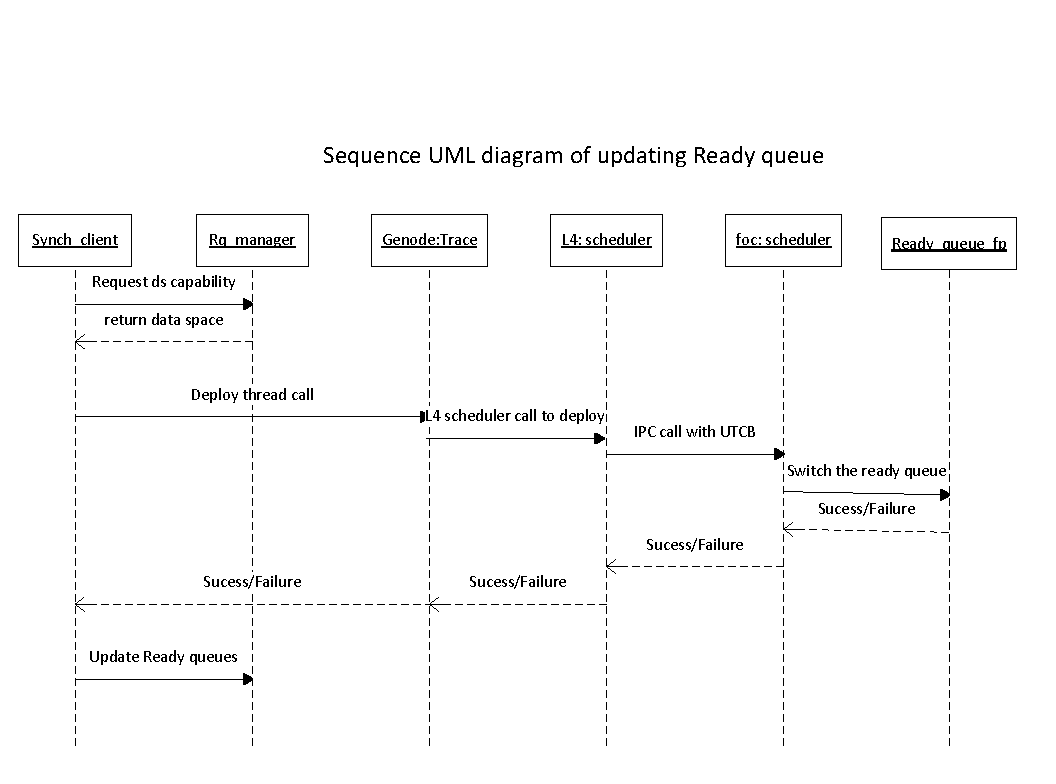
\includegraphics[width=1.0\linewidth]{figures/sequence_classUpdate}
\caption{Sequence diagram of updating ready queue from the Genode component}
\label{fig:sequence_classUpdate}
\end{figure}

\section{Rq\_manager Module}

 The class \texttt{Rq\_manager} is the driver class of this component. It creates and maintains multiple ready queues at the user-level component, where each queue is of type Rq\_buffer. The Rq\_buffer is a template class, which implements a circular array by using the Genode dataspace. Each entry in the Genode dataspace is a circular array of type Rq\_task struct, which represents a Genode thread.

The code listing \ref{rqmanager} shows the implementation of the \texttt{Rq\_manager} class. The constructor of \texttt{Rq\_manager} class first gets the number of available cores from Monitoring agent, then the \texttt{\_init\_rq()} function initializes the ready queues by using \texttt{init\_w\_shared\_ds} method from the Rq\_buffer class. The \texttt{Rq\_manager} provides enqueue and dequeue operations for the manipulation of the ready queue.

\begin{lstlisting}[caption={Rq\_manager class},label={rqmanager}, style=customcpp]
class Rq_manager
{	

		private:

			int _num_cores = 0;
			Rq_buffer<Rq_task> *_rqs; /* array of ring buffers (Rq_buffer with fixed size) */
			
			int _set_ncores(int);

		public:

			int enq(int, Rq_task);
			int deq(int, Rq_task**);
			int get_num_rqs();
			Genode::Dataspace_capability get_core_rq_ds(int);

			Rq_manager()
			{
				PINF("Value of available system cores not provided -> set to 2.");

				_set_ncores(2);
				_init_rqs(100);
			}

			_init_rqs(int rq_size)
			{

				_rqs = new Rq_buffer<Rq_task>[_num_cores];

				for (int i = 0; i < _num_cores; i++) {
					_rqs[i].init_w_shared_ds(rq_size);
				}
				Genode::printf("New Rq_buffer created. Starting address is: %p.\n", _rqs);

				return 0;

			}
}
\end{lstlisting}

The Rq\_buffer is a template class, which represents the ready queue on the application side. It implements a circular array with a fixed size. It uses the \texttt{head} pointer, which points to the beginning of the array and the \texttt{tail} pointer, which points to the end of the array. The elements are always inserted at the tail pointer and removed from the head. The pointers are wrapped around whenever they reach the end of the array. The free space available between the head and the tail is represented by using a pointer called \texttt{window}. 

Rq\_buffer has enqueue and dequeue functionalities, which can be called by the \texttt{Rq\_manager} to insert or remove an element from the ready queue. It also provides a functionality to initialize and create a shared dataspace. The code listing \ref{rqbuffer} shows the process of allocating memory for the shared dataspace and attaching it to the RM session of the component.

\begin{lstlisting}[caption={Allocating dataspace},label={rqbuffer}, style=customcpp]

	Genode::Dataspace_capability _ds; /* dataspace capability of the shared object */
	char *_ds_begin = nullptr;        /* pointer to the beginning of the shared dataspace */

		/* 
		 * create dataspace capability, i.e. mem is allocated,
		 * and attach the dataspace (the first address of the
		 * allocated mem) to _ds_begin. Then all the variables
		 * are set to the respective pointers in memory.
		 */
	_ds = Genode::env()->ram_session()->alloc(ds_size);
	_ds_begin = Genode::env()->rm_session()->attach(_ds);

\end{lstlisting}

The code listing \ref{rqtask} shows the Rq\_task structure, which represents an entry in the ready queue buffer. It contains the parameters, such as task\_id that are used to identify a Genode task.

\begin{lstlisting}[caption={Rq\_task structure},label={rqtask}, style=customcpp]
 struct Rq_task
 	{
 
			unsigned long task_id;
 			int wcet;
 			bool valid;
 
 	};
\end{lstlisting}

The access to this shared dataspace must be synchronized, since both the \texttt{Controller} and the \texttt{Synch\_client} use it. This is done using the locks provided by the Genode.

\section{Synch\_client Module}
The \texttt{Synch\_client} class represents a Genode component that controls the process of the scheduler ready queue update. It acts as a client in the Genode by using the services of the \texttt{Rq\_manager} and accesses the shared dataspace. The \texttt{Controller} and the \texttt{Synch\_client} interaction is that of a producer-consumer relationship. The producer (\texttt{Controller}) decides and produces (puts it in a buffer) a thread that needs to be executed, and a consumer(\texttt{Synch\_client}) picks the threads to the kernel ready queue.

The initial communication with the \texttt{Rq\_manager} is governed by an RPC call. In order to make an RPC call, it creates a Connection object. The following pointers are used for manipulating the circular buffer:

\begin{labeling}{pointers}
	\item [\_rqbufp] Hold the pointer to the Rq\_buffer type
	\item [\_lock] Lock needed to ensure mutual exclusion
	\item [\_head] Head pointer, points to the start of the Rq\_buffer
	\item [\_tail] Tail pointer, points to end of the Rq\_buffer
	\item [\_window] The window of free spaces available in between the head and the tail
\end{labeling}
 
There can be more than one ready queue. So, we need multiple pointers of each type. The data type \texttt{vector} is used to represent the pointers, since the available number of ready queues is unknown at the time of creation. The declaration of all the data structures are shown in Listing \ref{synchdata}. 

\begin{lstlisting}[caption={Data structures used in Synch\_client},label={synchdata}, style=customcpp]
	Rq_manager::Connection rqm;
	
	/* using vectors since we dont know the size initially */
	std::vector<int *> _rqbufp;
	std::vector<int *> _lock;
	std::vector<int *> head; 
	std::vector<int *> tail; 
	std::vector<int *> window;
	
	std::vector<Dataspace_capability> dsc;
	std::vector<Rq_manager::Rq_task*> buf;
\end{lstlisting}

We can use the Connection object created to make RPC calls to the\texttt{Rq\_manager}. The first RPC call is to obtain the number of ready queues available. For each ready queue available, the Connection object has to make an RPC call to get the dataspace capability, attach to the local RM session and initialize all the pointers shown in Listing \ref{synchdata}. 

\begin{figure}[h]
\centering
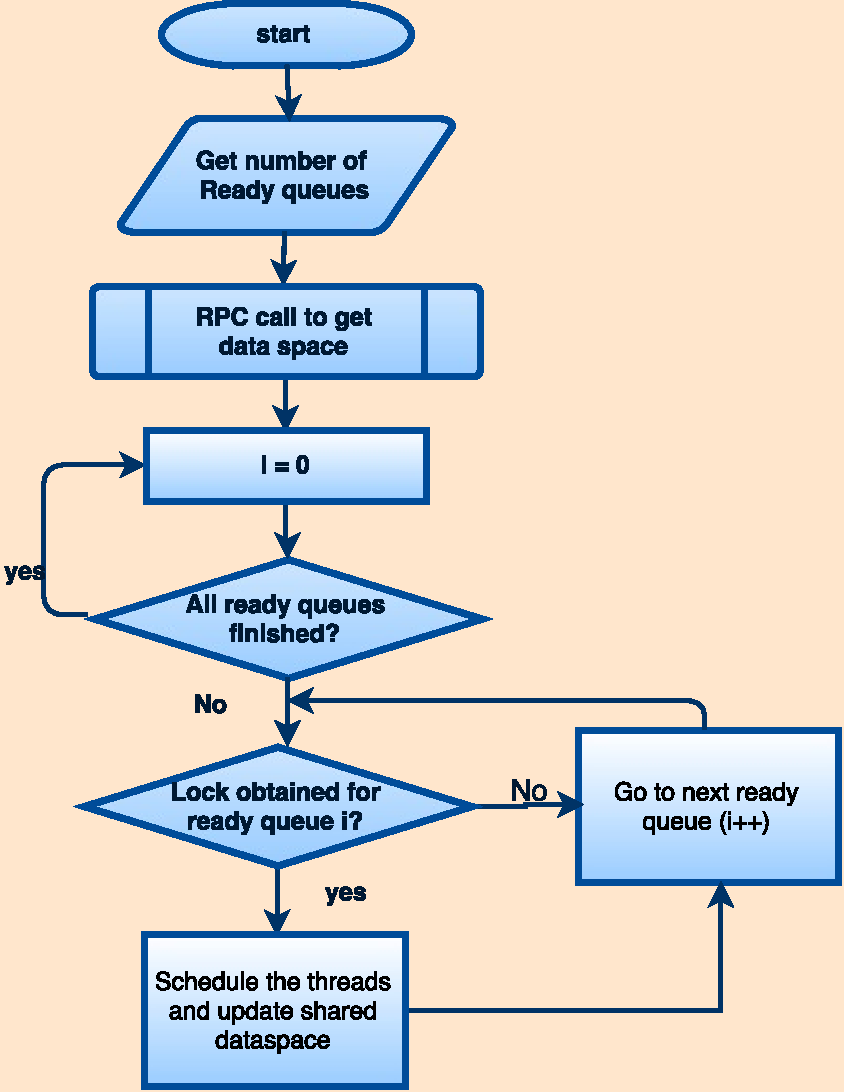
\includegraphics[width=0.5\linewidth]{figures/flow}
\caption{The execution of Synch\_client module}
\label{fig:flow}
\end{figure}

The working flow of the the \texttt{Synch\_client} module can be seen in Figure \ref{fig:flow}. After everything has been initialized, the \texttt{Synch\_client} runs in an infinite loop. For each ready queue, it tries to obtain the lock. If the locking is successful, it schedules the threads available in the ready queue. The infinite loop has two goals. First, it has to ensure that it moves on to the next ready queue so that the threads in other queues also get scheduled. Second, it has to reduce the amount of time spent in the critical section as to little as possible. In order to achieve the above mentioned goals, the ids of the threads/tasks are copied to a local buffer, the head and tail pointers updated and the lock is released. In this way, the scheduling of threads by calling the Genode API is kept outside the critical section.

One more option to reduce the critical section is to have separate threads working on each of the ready queues. If each thread works on a different ready queue, there is no shared data between these threads, and this guarantees the second goal mentioned for the infinite loop. 
 
\section{Ready Queue Update Mechanism}

The ready queue update mechanism follows the series of calls, which are shown in sequence diagram Figure \ref{fig:Drawing2}. The following subsections explain the implementation of the modules described in Figure \ref{design:rqupdate}.

\begin{figure}[h]
\centering
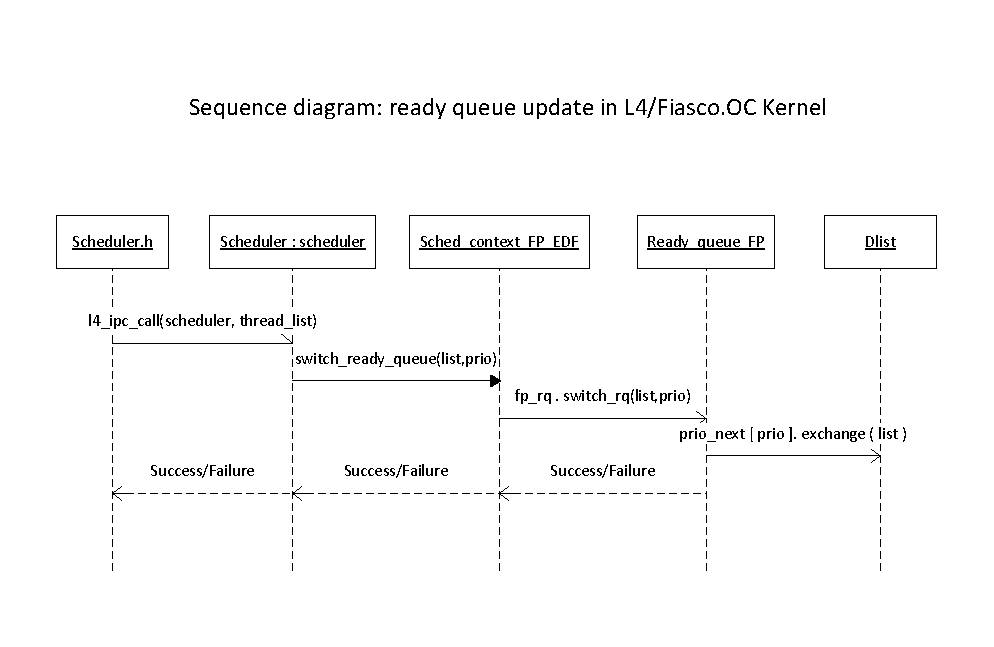
\includegraphics[width=1.0\linewidth]{figures/Drawing2}
\caption{}
\label{fig:Drawing2}
\end{figure}

\subsection{Genode Code Changes}

The Genode should provide a way to the application for calling the L4 API calls. In the present Genode code, the L4 APIs calls for scheduling threads are done from \texttt{Platform\_thread.cpp}, where the thread gets created. But, the \texttt{Platform\_thread} is not accessible from the application, as it doesn't provide any RPC interface for applications to make use of its services. The only way that the components communicate in Genode is by using RPC calls. So, an RPC call needs to be provided for the components to use it. As of now, this call is kept in the \texttt{Trace} service. The \texttt{Trace} service is used by the monitoring agent already to obtain the data from the Genode. The Trace service has been extended to provide an API, which can be used from the \texttt{Synch\_client} component to access the L4 APIs.

The \texttt{base/src/trace/trace\_session\_component.cc} contains the API definition, in which it takes a structure argument of threads and calls the L4 scheduler call.

\subsection{L4 API Calls} \label{imp:l4api}
This thesis introduces a new L4 API, which can be called from the Genode. The APi takes the following arguments:

\begin{itemize}
\item l4\_cap\_idx\_t: It takes a kernel object, which is the scheduler object.  

\item l4\_sched\_thread\_list: This is a structure, which can be seen in \ref{l4api} and has an array to hold the list of threads and the priorities for the same threads. 

\end{itemize}

Listing \ref{l4api} shows the l4\_sched\_thread\_list structure and the L4 API call, which is called from Genode. This code is present in \texttt{foc/l4/l4sys/scheduler.h}.
\begin{lstlisting}[caption={L4 scheduler API in scheduler.h},label={l4api}, style=customcpp]

typedef struct l4_sched_thread_list
{
	l4_cap_idx_t list[10];
	unsigned prio[10];
	int n;
}l4_sched_thread_list;

L4_INLINE l4_msgtag_t
l4_scheduler_deploy_thread(l4_cap_idx_t scheduler,
		l4_sched_thread_list thread) L4_NOTHROW
{
  return l4_scheduler_deploy_thread_u(scheduler, thread, l4_utcb());
}
\end{lstlisting}

The deploy thread function call has to fill the UTCB message registers and make an IPC call to the scheduler kernel object. The first register (mr[0]) is populated with the type of operation that the scheduler should do perform with the information. In this project, it is L4\_SCHEDULER\_DEPLOY\_THREAD\_OP. The second register is populated using a call to l4\_map\_obj\_control function, which returns a word. This word identifies the kernel objects, which come after this word in the message registers. After the map object control word is filled, thread objects are filled in the message registers in the form of L4 flex pages. An L4 flex page represents a naturally aligned area of mappable space, such as memory, I/O-ports and capabilities (kernel objects). In this project, L4 flex represents a thread object.
For each thread id that is sent, an L4 flex page is created and stored in the UTCB message registers. The L4 API makes an IPC call to the kernel scheduler object. 

Listing \ref{l4apimp} shows the L4 scheduler API implementation.

\begin{lstlisting}[caption={L4 scheduler API implementation},label={l4apimp}, style=customcpp]
L4_INLINE l4_msgtag_t
l4_scheduler_deploy_thread_u(l4_cap_idx_t scheduler, l4_sched_thread_list thread,
			  l4_utcb_t *utcb) L4_NOTHROW
{
  l4_msg_regs_t *m = l4_utcb_mr_u(utcb);
  m->mr[0] = L4_SCHEDULER_DEPLOY_THREAD_OP;
  m->mr[1] = l4_map_obj_control(0, 0);

  for(int i = 0; i < thread.n; i++){
	  m->mr[i+1] = l4_obj_fpage(thread.list[i], 0, L4_FPAGE_RWX).raw;
  }
  
  return l4_ipc_call(scheduler, utcb, l4_msgtag(L4_PROTO_SCHEDULER, thread.n+1, 1, 0), L4_IPC_NEVER);
  }
\end{lstlisting}
  
\section{Fiasco.OC Code Changes}
Fiasco.OC code changes are made in several files to incorporate the ready queue update mechanism in the kernel. The following sections explain the code changes in each file.

\subsection{Scheduler Class}

The \texttt{l4\_ipc\_call} from scheduler.h invokes the \texttt{kinvoke} function. The first parameter of the UTCB is decoded to find out the operation that the thread is involved in. The operation in this case was set to \texttt{deploy\_thread}, which calls the function \texttt{sys\_deploy\_thread} and can be seen in Listing \ref{sysdeploycode}. A for loop to get the number of available threads is executed. The associated flex page is derived from the sent items and a lookup is performed to obtain the thread objects. The thread objects can be used to obtain the scheduler context that they are associated with. The scheduler context objects are used to create a ready queue list(Fp\_list). This list is used to switch the actual ready queue of the scheduler.

The specified ready queue of the CPU can be obtained if the CPU was specified from the \texttt{Controller}. Otherwise, the ready queue of the thread's home CPU can be used. The current implementation creates and works with a fixed priority list. However, this can be extended easily to create the corresponding ready queue list. If there is only one thread, the \texttt{ready\_enqueue} function can be called instead of exchanging the complete list.


\begin{lstlisting}[caption={Thread extraction and ready list creation},label=sysdeploycode, style=customcpp]
Scheduler::sys_deploy_thread(L4_fpage::Rights, Syscall_frame *f, Utcb const *utcb)
{
	printf("[Scheduler: sys_deploy_thread] 1\n");
	L4_msg_tag const tag = f->tag();
	Cpu_number const curr_cpu = current_cpu();

	Obj_space *s = current()->space();
	assert(s);

	typedef Sched_context::Fp_list List;

	List list;
	
	for(int i = 6 ; i <= tag.words(); i++){
				
				/*
				 *	Get the messages in an iterator
				 */
				L4_snd_item_iter snd_items(utcb, i);

				/*
				 * Check if the items exist
				 */
				if (EXPECT_FALSE(!tag.items() || !snd_items.next()))
					return commit_result(-L4_err::EInval);

				L4_fpage _thread(snd_items.get()->d);

				if (EXPECT_FALSE(!_thread.is_objpage()))
					return commit_result(-L4_err::EInval);

				/*
				 * Do a look up to get the corresponding thread and cast 
				 * it to Thread_object type
				 */
				Thread *thread = Kobject::dcast<Thread_object*>(s->lookup_local(_thread.obj_index()));
				if (!thread)
					return commit_result(-L4_err::EInval);

				printf("[Scheduler:sys_deploy] Thread to be scheduled: %lx\n", thread->dbg_id());

				list.push(thread->sched_context(), List::Front);

				Sched_context::Ready_queue &rq = Sched_context::rq.cpu(thread->home_cpu());

				if(i==tag.words()){
				 rq.switch_ready_queue(&list, 100);
				}
		}
}
\end{lstlisting}

\subsection{Ready\_queue\_base Class}

This class implements the major functionalities to handle the ready queues. This class contains the lists of both FP ready queue and EDF ready queue and serves as a wrapper class to both type of lists. Any call made to access either of the ready queues goes through this class. The decision to call the specific ready queue function is made according to the type of the scheduler in use.

Since this work was involved with fixed priority lists, the check to find out the type of scheduler is excluded and the FP ready queue is used by default. However, it can be extended easily to work with both the lists. Listing \ref{switchrq} shows the calling of the function to fixed priority ready queue.

\begin{lstlisting}[caption={Exchanging the ready queue},label=switchrq, style=customcpp]
IMPLEMENT
bool
Sched_context::Ready_queue_base::switch_rq(Fp_list *list, unsigned prio)
{
	return fp_rq.switch_rq(list, prio);
}
\end{lstlisting}

\section{Synchronization Method}\label{imp:sync}

The ready queue contains the scheduler contexts that are part of the threads and can be run next. Modifying the ready queue list is a critical section operation and mutual exclusive access must be guaranteed. In a uniprocessor implementation, this can work with a simple CPU lock operation, which disables the interrupts on the local CPU so that no other threads can get CPU time in the middle of a ready queue manipulation. For SMP systems, the kernel must use a ready list local to the CPU. The Fiasco.OC implements a per-CPU variable that is used for synchronizing the ready queue access. When using per-CPU variable, the exclusive access to this variable is guaranteed by disabling the CPU preemption. Once this access is finished, the CPU preemption is enabled. By this way, if any CPU is in the middle of a critical section, no other thread is allowed to replace the current thread's execution on the CPU. 

The present method uses the per-CPU variable method in which it locks the CPU before exchanging the ready queue list. The Software Transactional Memory(STM) method was implemented, but testing it was a problem because using STM forces the GCC compiler to employ the pthreads library, which was not possible to include for the Fiasco.OC. The STM method will eliminate the need to preempt the CPU since it executes all the exchange instructions in one transaction.

A check is made in scheduler.cpp to find out if the ready queue is empty. If the ready queue is empty or contains the idle thread, then the immediate call is made to exchange the list. The \textit{static point-in-time} method checks if a thread from this ready list is getting executed. If the thread is running, the exchange call waits till the scheduler takes the control back and exchanges the thread list. This method uses the  \texttt{schedule\_in\_progress} flag to check if the scheduler is busy.

\subsection{Smart-Sync Method}
Finding the suitable time to update the ready queue is explained in section \ref{design:time}. The implementation of it is termed as \texttt{Smart-Sync} method. The \textit{Empty ready-queue} method is implemented by checking the running queue in the Scheduler class. The second method, \textit{Static point-in-time} is implemented by checking the scheduler business and this can be seen in Listing \ref{smart}.  

\begin{lstlisting}[label={smart}, style=customcpp]
/*
 * Empty ready-queue method
 */
if(ready_empty(prio)) {
	rq.switch_ready_queue(&list, prio);
}

/*
 * Static point-in-time method
 */
while(scheduler_in_use) { //Do nothing}
rq.switch_ready_queue(&list, prio);


\end{lstlisting} 

\subsection{Ready\_queue\_fp Class} \label{imp:rqfp}
From here on, the list that is sent is referred as new list and the list to be exchanged is referred as old list. Once the fixed priority ready queue is decided to be exchanged, the new list and the priority are sent to the \texttt{switch\_rq} function from the sched\_context-fp\_EDF class. It is assumed at this point that the new list contains the system threads, such as the idle and pager threads that are necessary to execute other threads. The Fiasco.OC uses an idle thread, which keeps the CPU busy when there are no threads to be executed. The idle thread needs to be kept in the new list if it is not existing already. The old list can be used to identify the idle thread, which sits in the end of the old list.

The exchange of the list is a simple operation of changing the head pointers. The cyclic list is implemented in a file called \texttt{dlist}. The \texttt{exchange} function was implemented to take the list to be exchanged with the present list and set the head of the old list to the new list. 

Listing \ref{rq_exchange} shows the \texttt{switch\_rq} function.

 \begin{lstlisting}[caption={Exchanging the ready queue},label=rq_exchange, style=customcpp]
 bool switch_rq(List *list, unsigned prio) {
   		assert_kdb(cpu_lock.test());
 
   		prio_next[prio].exchange(list);
 
   		//prio_next[prio].rotate_to(*++List::iter(list->front()));
 
   		typename List::BaseIterator it = List::iter(prio_next[prio].front());
   		dbgprintf("After exchange fp_rq: ");
   		do
   		{
   			dbgprintf("%lx => ",Kobject_dbg::obj_to_id(it->context()));
   		}while (++it != List::iter(prio_next[prio].front()));
   		dbgprintf("end\n");
 
   		return true;
   	}
 
\end{lstlisting}

\section{Implementation Challenges}
This section describes the challenges that were faced during the implementation phase and the how these challenges were overcome.

\subsection{Mapping the Threads from the Genode to the Kernel}
The threads are represented differently in the Genode OS framework and in the Fiasco.OC kernel. This was a problem while mapping the threads from the user-space to the kernel-space. A thread object can be identified by the integer ids of type \textit{unsigned long} that they carry. However, these differ between the user-space and the kernel-space. The \texttt{thread\_base} class in Genode has a native thread id, but it is not the same as the one represented in the kernel.

To identify the kernel id, the thread creation model was followed to check the mapping process. This happens in the L4 layer and the Scheduler class as explained in Section \ref{imp:l4api}.

%As explained before the Genode creates object-identities in kernel space when it creates an RPC object in the Genode (see \ref{Foundations:cap}). So the threads in Geno

\subsection{Sending Threads to the Kernel Module}
The thread ids and their priorities have to be sent to the kernel module from the user-space application in order to execute them. the thread ids can be sent one at a time, but this slows down the process because the calls have to be made for each thread id. The dynamic array creation also doesn't work since the user-space memory cannot be accessed in the kernel-space. 

The solution was to use a structure which has an array for thread ids and an array for the corresponding priorities. This structure is defined in the \textit{L4/scheduler.h} file (see \ref{imp:l4api}).

\subsection{Exchanging the Ready Queue}
The ready queue list is sent from the \texttt{Scheduler} object to the \texttt{Ready\_queue\_fp} class for to be exchanged. The swapping is not possible by just assigning the new list address to the old list address because it doesn't ensure the validity of the list since the head pointer of the list is not assigned. The solution is to assign the head pointer of the old list to the new list (see \ref{imp:rqfp}).